\documentclass[dvipsnames, hidelinks]{beamer}

% Enables the use of colour.
\usepackage{xcolor}
% Syntax high-lighting for code. Requires Python's pygments.
\usepackage{minted}
% Enables the use of umlauts and other accents.
\usepackage[utf8]{inputenc}
% Diagrams.
\usepackage{tikz}
% Settings for captions, such as sideways captions.
\usepackage{caption}
% Symbols for units, like degrees and ohms.
\usepackage{gensymb}
% Latin modern fonts - better looking than the defaults.
\usepackage{lmodern}
% Allows for columns spanning multiple rows in tables.
\usepackage{multirow}
% Better looking tables, including nicer borders.
\usepackage{booktabs}
% More math symbols.
\usepackage{amssymb}
% More math layouts, equation arrays, etc.
\usepackage{amsmath}
% More math fonts, like mathbb.
\usepackage{amsfonts}
% More theorem environments.
\usepackage{amsthm}
% More column formats for tables.
\usepackage{array}
% Adjust the sizes of box environments.
\usepackage{adjustbox}
% Better looking single quotes in verbatim and minted environments.
\usepackage{upquote}
% Better blank space decisions.
\usepackage{xspace}
% Better looking tikz trees.
\usepackage{forest}
% URLs.
\usepackage{hyperref}
% For plotting.
\usepackage{pgfplots}

% Various tikz libraries.
% For drawing mind maps.
\usetikzlibrary{mindmap}
% For adding shadows.
\usetikzlibrary{shadows}
% Extra arrows tips.
\usetikzlibrary{arrows.meta}
% Old arrows.
\usetikzlibrary{arrows}
% Automata.
\usetikzlibrary{automata}
% For more positioning options.
\usetikzlibrary{positioning}
% Creating chains of nodes on a line.
\usetikzlibrary{chains}
% Fitting node to contain set of coordinates.
\usetikzlibrary{fit}
% Extra shapes for drawing.
\usetikzlibrary{shapes}
% For markings on paths.
\usetikzlibrary{decorations.markings}
% For advanced calculations.
\usetikzlibrary{calc}

% GMIT colours.
\definecolor{gmitblue}{RGB}{20,134,225}
\definecolor{gmitred}{RGB}{220,20,60}
\definecolor{gmitgrey}{RGB}{67,67,67}

% Change some style options.
\usetheme{metropolis}
\usemintedstyle{manni}
\setbeamercolor{structure}{fg=gmitblue}
\setbeamercolor{frametitle}{fg=white, bg=gmitred}
\setbeamercolor{alerted text}{fg=gmitblue}
\usefonttheme[onlymath]{serif}

% \citeurl can be used to a clickable short url to a slide as a reference.
\renewcommand\footnoterule{}
\newcommand{\citeurl}[1]{\let\thefootnote\relax\footnotetext{\tiny \textcolor{gmitgrey}{\href{http://#1}{#1}}}}
\newcommand{\citeeg}[1]{\let\thefootnote\relax\footnotetext{\tiny \textcolor{gmitgrey}{#1}}}

% A basic horizontal rule.
\newcommand{\hr}{\rule{\textwidth}{0.5pt}}

% Prevent minted from showing errors.
\makeatletter
\expandafter\def\csname PYGdefault@tok@err\endcsname{\def\PYGdefault@bc##1{{\strut ##1}}}
\makeatother


% Change colours in tikz pictures.
\tikzset{onslide/.code args={<#1>#2}{%
  \only<#1>{\pgfkeysalso{#2}} % \pgfkeysalso doesn't change the path
}}
\tikzset{temporal/.code args={<#1>#2#3#4}{%
  \temporal<#1>{\pgfkeysalso{#2}}{\pgfkeysalso{#3}}{\pgfkeysalso{#4}} % \pgfkeysalso doesn't change the path
}}


\begin{document}
  \title{Finite Automata}
  \subtitle{}
  \author{ian.mcloughlin@gmit.ie}
  \date{}

  \begin{frame}
    \titlepage
  \end{frame}

  \begin{frame}[fragile]{Finite Automaton: Example 1}
  \begin{center}
    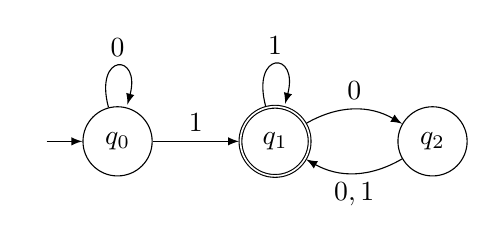
\begin{tikzpicture}[auto, on grid, node distance=2cm, initial text=, >=latex]
      \node[state, initial]   (q_0)                {$q_0$}; 
      \node[state, accepting] (q_1) [right of=q_0] {$q_1$};
      \node[state]            (q_2) [right of=q_1] {$q_2$}; 
      \path[->] 
        (q_0) edge [loop above] node {$0$}   ()
              edge []           node {$1$}   (q_1)
        (q_1) edge [bend left]  node {$0$}   (q_2)
              edge [loop above] node {$1$}   ()
        (q_2) edge [bend left]  node {$0,1$} (q_1);
    \end{tikzpicture}
  \end{center}
  \pause
  \begin{center}
    Try running the automaton on the following strings. \\
    $1101$, $1$, $01$, $11$, $0101010101$, $100$, $0100$, \\
    $110000$, $0101000000$, $0$, $10$, $101000$
  \end{center}
  \citeeg{Sipser page 34}
\end{frame}


\begin{frame}[fragile]{Finite Automaton: Example 2}
  \begin{center}
    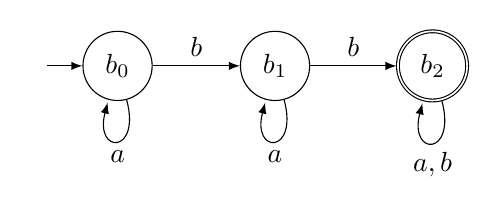
\begin{tikzpicture}[auto, on grid, node distance=2cm, initial text=, >=latex]
      \node[state, initial]   (b_0)                {$b_0$}; 
      \node[state]            (b_1) [right of=b_0] {$b_1$};
      \node[state, accepting] (b_2) [right of=b_1] {$b_2$}; 
      \path[->] 
        (b_0) edge [loop below] node {$a$}   ()
              edge []           node {$b$}   (b_1)
        (b_1) edge [loop below] node {$a$}   ()
              edge []           node {$b$}   (b_2)
        (b_2) edge [loop below] node {$a,b$} ();
    \end{tikzpicture}
  \end{center}
  \pause
  \begin{center}
    Try running the automaton on the following strings. \\
    $aaaa$, $ababa$, $bababb$, $abaa$ \\
    \pause
    \vspace{8mm}
    Describe the strings that the automaton recognises.
  \end{center}
  \citeeg{Sipser chapter 1 4(a) -- Part 2}
\end{frame}

\begin{frame}[fragile]{Finite Automaton: Example 3}
  \begin{center}
    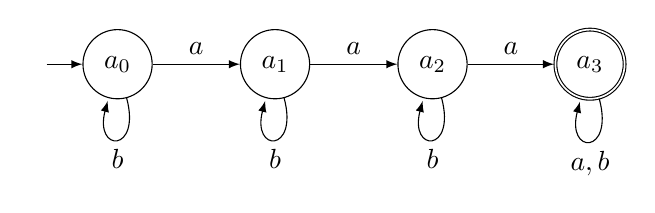
\begin{tikzpicture}[auto, on grid, node distance=2cm, initial text=, >=latex]
      \node[state, initial]   (a_0)                {$a_0$}; 
      \node[state]            (a_1) [right of=a_0] {$a_1$};
      \node[state]            (a_2) [right of=a_1] {$a_2$}; 
      \node[state, accepting] (a_3) [right of=a_2] {$a_3$};
      \path[->] 
        (a_0) edge [loop below] node {$b$}   ()
              edge []           node {$a$}   (a_1)
        (a_1) edge [loop below] node {$b$}   ()
              edge []           node {$a$}   (a_2)
        (a_2) edge [loop below] node {$b$}   ()
              edge []           node {$a$}   (a_3)
        (a_3) edge [loop below] node {$a,b$} ();
    \end{tikzpicture}
  \end{center}
  \begin{center}
    \pause
    Try running the automaton on the following strings. \\
    $aaaa$, $ababa$, $bababb$, $abaa$ \\
    \vspace{8mm}
    \pause
    Describe the strings that the automaton recognises.
  \end{center}
  \citeeg{Sipser chapter 1 4(a) -- Part 1}
\end{frame}

\begin{frame}[fragile]{Finite Automaton: Concepts}
  \begin{center}
    \begin{tikzpicture}[auto, on grid, node distance=2cm, initial text=, >=latex]
      \node[state, initial, onslide={<2,3>{gmitblue}}]   (q_0)                {$q_0$}; 
      \node[state, accepting, onslide={<2,4>{gmitblue}}] (q_1) [right of=q_0] {$q_1$};
      \node[state, onslide={<2>{gmitblue}}]              (q_2) [right of=q_1] {$q_2$}; 
      \path[->] 
        (q_0) edge [loop above, onslide={<6>{gmitblue}}] node {\only<5>{\textcolor{gmitblue}{$0$}} \only<1-4,6>{\textcolor{black}{$0$}}}   ()
              edge [,           onslide={<6>{gmitblue}}] node {\only<5>{\textcolor{gmitblue}{$1$}} \only<1-4,6>{\textcolor{black}{$1$}}}   (q_1)
        (q_1) edge [bend left,  onslide={<6>{gmitblue}}] node {\only<5>{\textcolor{gmitblue}{$0$}} \only<1-4,6>{\textcolor{black}{$0$}}}   (q_2)
              edge [loop above, onslide={<6>{gmitblue}}] node {\only<5>{\textcolor{gmitblue}{$1$}} \only<1-4,6>{\textcolor{black}{$1$}}}   ()
        (q_2) edge [bend left,  onslide={<6>{gmitblue}}] node {\only<5>{\textcolor{gmitblue}{$0,1$}} \only<1-4,6>{\textcolor{black}{$0,1$}}} (q_1);
    \end{tikzpicture}
  \end{center}

  \begin{center}
    \only<1>{\textcolor{gmitblue}{What are the essential concepts?}}
    \only<2>{\textcolor{gmitblue}{Set of states: $Q = \{ q_0, q_1, q_2 \}$}}
    \only<3>{\textcolor{gmitblue}{Initial state: $q_0 \in Q$}}
    \only<4>{\textcolor{gmitblue}{Set of final states: $F = \{ q_1 \} \subseteq Q$}}
    \only<5>{\textcolor{gmitblue}{Alphabet: $\Sigma = \{ 0, 1 \}$}}
    \only<6>{\textcolor{gmitblue}{Transition function: $\delta = \{ ((q_0, 0), q_0), ((q_0, 1), q_1), ((q_1,0), q_2), \ldots \}$}}
  \end{center}
\end{frame}


\begin{frame}[fragile]{Deterministic Finite Automaton (DFA) definition}
  A DFA is a 5-tuple $(Q,\Sigma,\delta,q_0,F)$ where
  \begin{description}
    \item[$Q$] is a finite set of \emph{states},
    \item[$\Sigma$] is a finite set called the \emph{alphabet},
    \item[$\delta$] is the \emph{transition function} ($Q \times \Sigma \rightarrow Q$),
    \item[$q_0$] is the \emph{start state} ($\in Q$), and
    \item[$F$] is the set of \emph{accept states} ($\subseteq Q$). 
  \end{description}
  \citeeg{Sipser page 35}
\end{frame}


\begin{frame}[fragile]{Example 1 definition}
  \begin{description}
    \item[$Q =$] $\{ q_0, q_1, q_2\}$
    \item[$\Sigma =$] $\{ 0, 1 \}$
    \item[$\delta =$] $\{ ((q_0,0),q_0), ((q_0,1),q_1)$, $((q_1,0),q_2), ((q_1,1),q_1)$, $((q_2,0),q_1), ((q_2,1),q_1) \}$
    \item[$q_0 =$] $q_0$
    \item[$F =$] $\{ q_1 \}$
  \end{description}
  \citeeg{Sipser page 36}
\end{frame}

\begin{frame}[fragile]{Example 2 definition}
  \begin{description}
    \item[$Q =$] $\{ b_0, b_1, b_2\}$
    \item[$\Sigma =$] $\{ a, b \}$
    \item[$\delta =$] $\{ ((b_0,a),b_0), ((b_0,b),b_1)$, $((b_1,a),b_1), ((b_1,b),b_2)$, $((b_2,a),b_2), ((b_2,b),b_2) \}$
    \item[$q_0 =$] $b_0$
    \item[$F =$] $\{ b_2 \}$
  \end{description}
  \citeeg{Sipser chapter 1 4(a) -- Part 1}
\end{frame}

\begin{frame}[fragile]{Example 3 definition}
  \begin{description}
    \item[$Q =$] $\{ a_0, a_1, a_2, a_3 \}$
    \item[$\Sigma =$] $\{ a, b \}$
    \item[$\delta =$] $\{ ((a_0,a),a_1), ((a_0,b),a_0)$, $((a_1,a),a_2), ((a_1,b),a_1)$, $((a_2,a),a_3), ((a_2,b),a_2) \}$, $((a_3,a),a_3), ((a_3,b),a_3) \}$
    \item[$q_0 =$] $a_0$
    \item[$F =$] $\{ a_3 \}$
  \end{description}
  \citeeg{Sipser chapter 1 4(a) -- Part 1}
\end{frame} 
\end{document}
 